\chapter{MARCO TEÓRICO}
\section{MARCO CONCEPTUAL}
\subsection{LeapMotion}

En los últimos años, se han desarrollado diferentes sensores de tipo óptico, que permiten la interacción con objetos 3D. Paralelamente a la aparición de nuevos sensores, que comunican el entorno real con el virtual también el número de aplicaciones relacionadas aumenta. Las aplicaciones se benefician especialmente de la precisión y robustez de los sensores 3D (Khoshelham K., Elberink S.O. Accuracy and resolution of kinect depth data for indoor mapping applications. Sensors) y debido al aumento de la producción de estos sensores se ha efectuado una baja en los precios. Las aplicaciones para sensores 3D incluyen tareas industriales, seguimiento de personas y objetos, análisis de movimiento, animación de personajes, reconstrucción de escenas 3D e interfaces de usuario basadas en gestos [Gesture Recognition using Microsoft Kinect. Proceedings of the IEEE International Conference on Automation]. Estas aplicaciones tienen diferentes requisitos en términos de resolución, velocidad, distancia y características de captura y particularmente con respecto a las interfaces de usuario basadas en gestos, la precisión del sensor es la tarea más desafiante. Los sensores de calidad para el consumidor ofrecen una precisión de posicionamiento limitada. Un análisis del controlador Kinect muestra una desviación estándar en la precisión de profundidad de aproximadamente 1,5 cm [Accuracy and resolution of kinect depth data for indoor mapping applications]. 





%\subsection{Goniometria}
%Lo goniometría es la ciencia que se ocupa de la medida angular. A pesar de que la goniometría se ha utilizado en varias disciplinas o, Para este proyecto es indispensable dar su uso en las ciencias de la salud en la que se usa para realizar la medición de movilidad articular en ángulos, ya sea enfocado a la evaluación preventiva, correctiva o exploratoria.


%\subsection{Análisis vectorial de la mano, antebrazo y muñeca}
%Esto es un modelo matemático de las entradas del leap motion no?

\subsection{Enfermedades y lesiones}
El \parencite{MinisteriodeProteccionSocialdeColombia2006GuiaSuperiores} define un Desorden Músculo Esquelético (DME) como una lesión física originada por trauma acumulado que se desarrolla gradualmente sobre un período de tiempo; como resultado de repetidos esfuerzos\footnote{Se entiende por “esfuerzos repetidos” a un grupo de movimientos continuos mantenidos durante un trabajo que implica la acción conjunta de (..) una parte del cuerpo y provoca en esta misma zona fatiga muscular, sobrecarga, dolor y, por último, lesión.\parencite{INSHT2016PrevencionRepetidos}} sobre una parte específica del sistema músculo esquelético\footnote{Está constituido por los huesos del cuerpo, los músculos, los tendones, los ligamentos, las articulaciones, los cartílagos y otras clases de tejido conjuntivo.}. 

El Instituto Nacional de Seguridad e Higiene en el Trabajo (INSHT) de España ha publicado a lo largo de los años diversas fichas que contienen directrices para la decisión clínica en enfermedades profesionales (DDC) en las cuales se denota una estructura consistente (definición, sintomas, maniobras de exploración, pruebas diagnósticas, vulnerabilidad, actividades de riesgo, repercusión), que posee información completa y depurada acerca de las enfermedades prevalentes en los puestos de trabajo para manos, muñeca y antebrazo.

Considerando lo anterior, se procede a realizar un listado comprensivo de estas enfermedades, tomando como fuente primara de información las fichas expuestas por el INSHT.
 %referencia especialista de salud

\subsubsection{Tenosinovitis De Quervain}
\paragraph{¿Qué es?}
En España, el Instituto Nacional de Seguridad e Higiene en el Trabajo (INSHT) define la Tenosinovitis De Quervainn (TDQ) conocida como tenosinovitis estiloides radiales, como la inflamación de los tendones del pulgar a causa de movimientos repetitivos. \parencite[1]{INSHT2017TendinitisPulgar}

\begin{figure}[H]
    \centering
    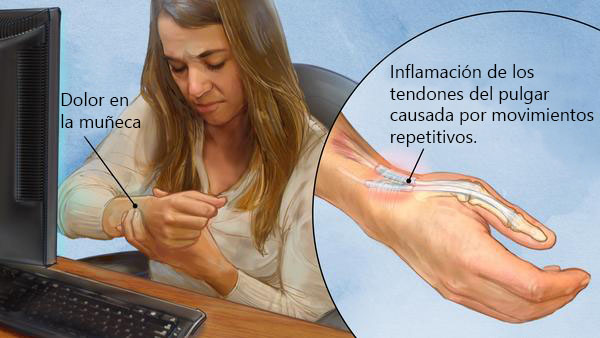
\includegraphics[width=0.7\textwidth]{Anexos/LATEX/chapters/images/TDQ.jpg}
    \caption{Análisis de la mano con Tenosinovitis de Quervain}
    \small{\textbf{Fuente:} https://g.co/kgs/BpkB4A}
    \label{TDQ}
\end{figure}

De acuerdo al \parencite[2]{INSHT2017TendinitisPulgar}, esta enfermedad se manifiesta como una inflamación que produce una estenosis del canal osteofibrososinovial situado en la estiloides radial por el que discurren los tendones del abductor largo y extensor corto del pulgar. Se produce al combinar agarres con giros o desviaciones cubitales y radiales repetidas o forzadas de la mano.
\paragraph{Repercusión}
La Enfermedad de Quervain (CIE-9 MC 727.04)\footnote{CIE-9-MC es un acrónimo de Clasificación Internacional de Enfermedades, Novena Revisión, Modificación Clínica. Se trata de una clasificación de enfermedades y procedimientos utilizada en la codificación de información clínica derivada de la asistencia sanitaria, principalmente en el entorno de hospitales y centros de atención médica especializada.} posee un tiempo estándar de incapacidad transitoria de 20 días.\parencite[6]{INSHT2017TendinitisPulgar}
\paragraph{Prevención}
Se aconseja no combinar agarres con giros o desviaciones cubitales y radiales repetidas. Para las situaciones de oficina que involucran un mouse, es necesario evitar realizar desplazamientos girando la muñeca, el movimiento adecuado debe ser desplazar el brazo en su totalidad desde el hombro. \parencite[5]{INSHT2017TendinitisPulgar}
\subsubsection{Síndrome del Túnel del Carpo}
\paragraph{¿Qué es?}
EL INSHT describe un espacio en la muñeca llamado túnel del carpo, a través del cual pasan el nervio mediano y nueve tendones flexores que van desde el antebrazo hacia la mano\parencite[1]{INSHT2017SindromeCarpiano}. Con base en lo anterior se define el Síndrome del Túnel del Carpo (STC) como una condición producida por la compresión del Nervio Mediano, a nivel de la muñeca. Esta compresión produce entumecimiento, hormigueo y dolor en la mano, dedos y ocasionalmente en el brazo. \parencite[1]{INSHT2017SindromeCarpiano}

\begin{figure}[H]
    \centering
    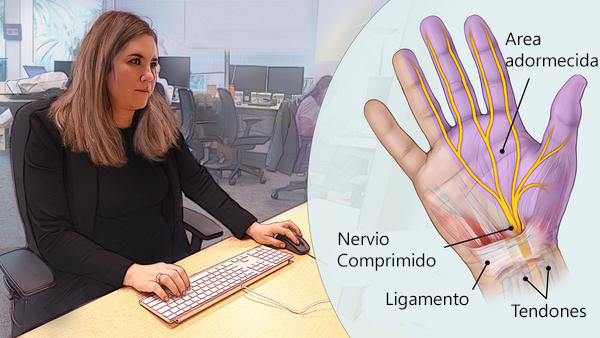
\includegraphics[width=0.7\textwidth]{Anexos/LATEX/chapters/images/STC.jpg}
    \caption{Análisis de la mano con Síndrome del Túnel del Carpo}
    \small{\textbf{Fuente:} https://g.co/kgs/MdPBTe}
    \label{STC}
\end{figure}

Siguiendo la definición dada por el \parencite{INSHT2017SindromeCarpiano}, el STC se presenta cuando se aumenta la presión dentro del túnel por cualquier proceso inflamatorio, comprimiendo el nervio, el cual es una estructura muy sensible a los aumentos de presión. Cuando la presión dentro del túnel es muy alta y altera la función normal del nervio, aparecen rigidez, hormigueo y dolor en la mano y los dedos.
\paragraph{Repercusión}
El Síndrome del Túnel Carpiano (CIE-9 MC 354.0) posee un tiempo estándar de incapacidad transitoria de 60 días\parencite[6]{INSHT2017SindromeCarpiano}.
\paragraph{Prevención}
Para evitar esta enfermedad la \parencite{FundacionSantaFedeBogota2016SindromeTratarlo} recomienda informar al trabajador, entrenándolo para que aquellas posturas o movimientos peligrosos sean evitados durante el desarrollo de su labor, además, el buen diseño de las herramientas, utensilios y del puesto de trabajo ayudan a conseguir la relajación de la mano y de la muñeca.

\subsubsection{Síndrome del túnel cubital}
\paragraph{¿Qué es?}
El \parencite[1]{INSHT2017SindromeCodo} describe esta enfermedad como una mononeuropatía \footnote{Es el daño a un solo nervio que produce pérdida del movimiento, la sensibilidad u otra función de dicho nervio. \parencite{MedlinePlus2018Mononeuropatia}} por compresión del nervio cubital cuando se hace superficial a nivel del codo.
\begin{figure}[H]
    \centering
    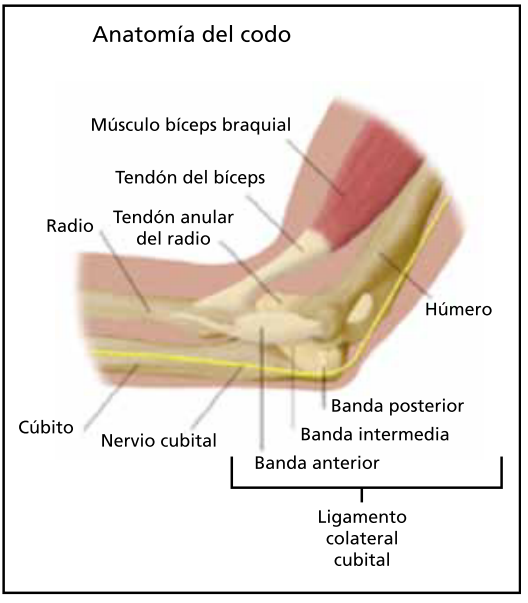
\includegraphics[width=0.4\textwidth]{Anexos/LATEX/chapters/images/AnaCodo.png}
    \caption{Análisis de la mano con Sindrome del túnel cubital}
    \small{\textbf{Fuente:} \parencite[1]{INSHT2017SindromeCodo}}
    \label{AnaCodo}
\end{figure}
\paragraph{Repercusión}
Una lesión del nervio cubital (CIE.9.MC: 352.2) posee un tiempo estándar de incapacidad transitoria de 60 días\parencite[6]{INSHT2017SindromeCodo}.
\paragraph{Prevención}
Evitar trabajos en los que se produzca un apoyo prolongado y repetido de forma directa o indirecta sobre las correderas anatómicas que provocan lesiones nerviosas por compresión, no realizar movimientos extremos de hiperflexión\footnote{Flexión forzada de una extremidad a un grado mayor de lo normal} y de hiperextensión\footnote{Posición en que se encuentra una articulación al sobrepasar su posición anatómica neutral} del codo.\parencite[5]{INSHT2017SindromeCodo}.


\section{MARCO REFERENCIAL}
\subsection{Modelos de valoración de riesgos posturales en Colombia}
\subsubsection{Normas GATI-SO}
Las Guías de Atención Integral de Salud Ocupacional Basadas en la Evidencia (GATI-SO) nacen a partir de un plan de trabajo propuesto por la dirección general de riesgos profesionales del ministerio de la protección social Colombiano con el objetivo de incrementar el diagnóstico y prevenir las enfermedades profesionales de
mayor prevalencia en Colombia \parencite[6]{MinisteriodeProteccionSocialdeColombia2006GuiaSuperiores}, esto se lleva a cabo a partir de la emisión de recomendaciones basadas en la evidencia.

Las características de los factores de riesgo ocupacional que han demostrado estar asociados con la aparición del \textbf{STC} son las siguientes:\parencite[45]{MinisteriodeProteccionSocialdeColombia2006GuiaSuperiores}
\begin{itemize}
\item Posturas en flexión y extensión de dedos, mano y muñeca, así como, la desviación ulnar o radial que implique agarre, pronación y supinación combinada con el movimiento repetitivo en ciclos de trabajo
\item Fuerza ejercida en trabajo dinámico por manipulación de pesos en extensión y flexión de los dedos y la mano
\item Vibración segmentaría derivada del uso de herramientas vibratorias
\end{itemize}
Las características de los factores de riesgo ocupacional que han demostrado estar asociados con la aparición del \textbf{TDQ} son las siguientes\parencite[45]{MinisteriodeProteccionSocialdeColombia2006GuiaSuperiores}:
\begin{itemize}
\item Postura forzada de muñeca asociada a movimiento de alta repetición (ciclos de tiempo menores a 30 segundos o 50 \% del ciclo gastado.
\end{itemize}
Adicionalmente se mencionan las siguientes conclusiones \parencite[46]{MinisteriodeProteccionSocialdeColombia2006GuiaSuperiores}:
\begin{itemize}
\item Existe evidencia de que las posturas asumidas de codo, antebrazo y mano se asocian con mayor frecuencia a los desórdenes de trauma acumulativo en población trabajadora.
\item Existe evidencia de que el movimiento repetitivo se asocia con mayor frecuencia a los desórdenes de trauma acumulativo en población trabajadora.
\item Existe evidencia de que la fuerza se asocia con mayor frecuencia a los desórdenes de trauma acumulativo en población trabajadora.
\end{itemize}
\subsection{Modelos de valoración de riesgos posturales internacionales}
A lo largo de los años se han consolidado diversas metodologías para realizar análisis de los factores de riesgo presentes en los puestos de trabajo, estas herramientas han sido estudiadas, consolidadas y depuradas por algunas entidades especializadas en la ergonomía en el trabajo. En la Universidad Politécnica de Valencia el grupo de investigación de ergonomía en el trabajo y prevención de riesgos laborales, conocido como Ergonautas (Dirigido por Phd. José Antonio Diego-Más), presenta un compendio de información que recopila todos los temas necesarios para realizar una correcta evaluación del puesto de trabajo. En cuanto a la evaluación de posturas, esta plataforma comprende una estructura estándar que facilita el entendimiento, la legibilidad y además proporciona una descripción enriquecida de los métodos tradicionales con bibliografía complementaria. 

Con base en lo anterior, Ergonautas representa una herramienta de apoyo útil para los objetivos de esta investigación, consolidándose como una de las fuentes primarias de información para las secciones presentadas a continuación.

\subsection{Método Rula}
El método RULA \textit{(Rapid Upper Limb Assessment)} tiene como objetivo de evaluar la exposición de los trabajadores a factores de riesgo que originan una elevada carga postural\footnote{Llevar a cabo posturas inadecuadas a manera continua o repetitiva que generen fatiga} y que pueden ocasionar trastornos en los miembros superiores del cuerpo. Para la evaluación del riesgo se consideran el método la postura adoptada, la duración, la frecuencia y las fuerzas ejercidas cuando se mantiene.\parencite[2]{Mcatamney1993RULA:Disorders}

El método RULA evalúa una determinada postura y esta obtiene una puntuación con base a los ángulos generados, estableciendo así un denomiando \textit{Nivel de Actuación}. El Nivel de Actuación indicará si la postura es aceptable o en qué medida son necesarios cambios o rediseños en el puesto. En resumen, RULA permite al evaluador detectar posibles problemas ergonómicos derivados de una excesiva carga postural.\parencite{Diego-Mas2015EvaluacionRULA}\parencite[4]{Mcatamney1993RULA:Disorders}

\parencite{Diego-Mas2015EvaluacionRULA} indica que RULA divide el cuerpo en dos grupos, el Grupo A que incluye los miembros superiores (brazos, antebrazos y muñecas) y el Grupo B, que comprende las piernas, el tronco y el cuello. Mediante las tablas asociadas al método, se asigna una puntuación a cada zona corporal (piernas, muñecas, brazos, tronco...) para, en función de dichas puntuaciones, asignar valores globales a cada uno de los grupos A y B.
\subsection{Método Reba}
REBA \textit{(Rapid Entire Body Assessment)} es un método basado en el previamente mencionado método RULA, diferenciándose fundamentalmente en la inclusión en la evaluación de las extremidades inferiores. Según \parencite{Diego-Mas2015EvaluacionREBA} REBA es uno de los métodos observacionales para la evaluación de posturas más extendido en la práctica.

Según expone \parencite{Hignett2000RapidREBA} REBA es un método de análisis postural acondicionado para evaluar las tareas que poseen cambios repentinos de postura, generalmente a causa de la manipulación de cargas inestables o impredecibles. Este método ayuda al evaluador a identificar los posibles riesgos relacionados a una postura, principalmente de tipo músculo-esquelético, orientando en cada circunstancia la inmediatez con la que se tienen que efectuar acciones correctivas.

\parencite{Diego-Mas2015EvaluacionREBA} resalta que el método REBA evalúa posturas individuales y no conjuntos o secuencias de posturas, por ello, recomienda seleccionar aquellas posturas que serán evaluadas de entre las que adopta el trabajador en el puesto. Luego, seleccionar aquellas que, a priori, supongan una mayor carga postural bien por su duración, bien por su frecuencia o porque presentan mayor desviación respecto a la posición neutra.
\subsection{Método Owas}
OWAS \textit{(Ovako Working Posture Analysing System)} es un sistema de evaluación de posturas de trabajo que analiza todas las posturas realizadas por el trabajador a lo largo de su jornada, con la ventaja de evaluar el riesgo de todas las posturas adoptadas de manera conjunta con base en la frecuencia y la gravedad.\parencite{MattilaMVilkki1999OccupationalSystems}

Este método es observacional, es decir, parte de la observación de las diferentes posturas adoptadas por el trabajador durante el desarrollo de la tarea a intervalos regulares \parencite{Diego-Mas2015EvaluacionOWAS}. Las posturas distinguidas son clasificadas en 252 posibles combinaciones dada la posición de los brazos, la espalda, y las piernas del trabajador, además, considera el peso con el que se realiza el movimiento. 

El autor citado anteriormente observó que como contrapartida, OWAS suministra estimaciones menos exactas, sin embargo, es la habilidad de contemplar un conjunto de posturas a través de la jornada laboral lo que consigue que OWAS siga siendo un método relevante a través de los años y continúe como uno de los más empleados en la evaluación de la carga postural.
\subsection{Método Ergo/IBV}
El método ERGO/IBV permite analizar tareas repetitivas de miembro superior con ciclos de trabajo claramente definidos, con el fin de evaluar el riesgo de lesión musculo esquelética en la zona del cuello-hombro y en la zona de la mano-muñeca.\parencite{Nogareda2009TareasErgonomicos}.

Para realizar una evaluación se requiere observar las posturas adoptadas por el trabajador, asignándoles un porcentaje que represente la cantidad de tiempo que ocupa esa actividad sobre el total, luego, se puntúa cada postura con respecto a el grado de inclinación desde la posición natural y finalmente se multiplica para ponderar el factor de riesgo.\parencite{Nogareda2009TareasErgonomicos}.
\section{MARCO TECNOLÓGICO}